\documentclass[10pt,a4paper]{article}
\usepackage{geometry}
\usepackage[french]{babel}
\usepackage[utf8]{inputenc}
\usepackage[T1]{fontenc}
\usepackage{lmodern} \normalfont
\DeclareFontShape{T1}{lmr}{bx}{sc}{<-> ssub * cmr/bx/sc}{}
\usepackage{textcomp}
\usepackage{datetime}
\usepackage{amsmath}
\usepackage{amssymb}
\usepackage{graphicx}
\usepackage{wrapfig}
\usepackage{subcaption}
\usepackage{tocloft}
\usepackage{fixltx2e}
\usepackage{color}
\usepackage[colorlinks=true,
			linkcolor=blue,
			bookmarksnumbered=true,
			pdftitle={Rapport INF4705},
			pdfauthor={Gwenegan Hudin},
			pdfborder={0 0 0},
			pdfsubject={Stage 3INFO}]{hyperref}

% Custom commands
\newcommand{\HRule}{\rule{\linewidth}{0.5mm}}
\newcommand{\Section}[1]{\section*{#1} \addcontentsline{toc}{section}{#1} \setcounter{subsection}{0}}
%\renewcommand*{\theHsection}{chY.\the\value{section}}
\renewcommand{\thesection}{\Roman{section}.}
\renewcommand{\thesubsection}{\arabic{subsection}.}
\renewcommand{\thesubsubsection}{\alph{subsubsection}.}
\renewcommand{\cftsecnumwidth}{2em}
\renewcommand{\cftsubsecnumwidth}{2em}
\renewcommand{\cftsubsubsecnumwidth}{2em}
\addto\captionsfrench{
	\renewcommand{\cfttoctitlefont}{\Large}
	\renewcommand{\contentsname}{\centering \textsc{Table des Matières}\\[0.5cm]}
}

\renewcommand{\baselinestretch}{1.15}

\begin{document}

\begin{titlepage}
	\begin{center}
		\begin{figure}
        \begin{subfigure}[c]{0.2\textwidth}
        		\centering
                
\includegraphics[width=0.6\textwidth]{images/logo-polymtl}
        \end{subfigure}
		\end{figure}
		
		
		\vspace{30pt}
		\textsc{\huge Génie Informatique}\\
		\textsc{\LARGE Rapport de Travaux Pratiques}\\		
		\vfill
		
		% Title
		\HRule \\[0.7cm]
		{\Huge \bfseries INF4705 : Lab 2}\\[0.4cm]
		{\Large Algorithmes voraces et dynamiques : Application au tri topologique d'un graphe}\\[0.2cm]
		\HRule\\[1cm]
		
		\vfill
		
		% Author
		\begin{minipage}{0.49\textwidth}
			\begin{flushleft} \LARGE
				\textbf{Auteur}\\
				Gwenegan \textsc{Hudin}\\ 1756642\\[0.5cm]
			\end{flushleft}
		\end{minipage}
		\begin{minipage}{0.49\textwidth}
			\begin{flushright} \LARGE
				\textbf{Rendu}\\
				14 Novembre 2014\\ À Polytechnique Montréal\\[0.5cm]
			\end{flushright}
		\end{minipage}
	\end{center}
\end{titlepage}

\newpage

\hfill

\newpage

\tableofcontents

\newpage

\section{Introduction}

Lors de cette expérience, nous allons couvrir le problème de tri topologique de graphes orientés acycliques selon trois approches : vorace, retour arrière et dynamique. Plus que les tris en eux-mêmes, nous nous intéresserons au nombre de permutations de tri détectées par chaque algorithme, et leurs vitesses respectives. Ces permutations seront nommées \og extensions linéaires \fg d'un graphe.

Au début de l'expérience, nous n'avons pas de suppositions de précédence d'une méthode sur une autre, et nous n'avons donc pas d'hypothèse précise à vérifier, contrairement au rapport précédent. Nous pouvons simplement supposer que l'algorithme vorace, dont l'utilisation afin de déterminer le nombre d'extensions linéaires repose sur une approximation par formule mathématique, sera moins précis que les deux autres méthodes.

L'on peut aussi supposer que l'algorithme de programmation dynamique, reposant sur une structure de données à $N$ dimensions, sera bien plus coûteux et difficile à implémenter, mais plus rapide que l'algorithme exhaustif de retour arrière.

Ce rapport a pour but de présenter les différents résultats obtenus avec chaque implémentation, appliquer des analyses asympotiques et hybrides, et de discuter des méthodes utilisées.

\section{Revue de la théorie}

Dans ce rapport, tous les graphes évoqués seront considérés orientés et acycliques, et définis formellement comme suit : $ G = (S,A) $, avec $S$ ensemble de sommets $\{1, \ldots, n\}$ et $A$ ensemble d'arcs tels que $ A \subset S \times S $.

On définit un tri topologique de $G$ comme étant une permutation $ \sigma $ de $ S $ telle que $ (i,j) \in A \longrightarrow \sigma(i) < \sigma(j) $.

Les trois méthodes reposent sur une mécanique similaire : détecter les sommets dont le degré entrant est nul, les traiter, les ignorer, itérer. Leur complexité théorique est étudiée plus tard dans ce rapport.

\subsection{Fonctionnement de l'algorithme vorace}

Contrairement aux deux autres méthodes que nous verrons, l'algorithme vorace ne vise pas directement l'obtention des extensions linéaires du graphe. 

Pour déterminer le nombre de permutations, l'algorithme calcule une décomposition du graphe en chaînes, de longueur décroissante. Ces chaînes sont calculées itérativement, en enlevant à chaque fois les sommets du graphe gérés.

Ensuite, cette décomposition permet d'approximer le nombre d'extensions linéaires selon $ 2^{ \frac{1}{2} n H(G)} $, où $ H(G) = \sum_{i=1}^{k} (- \frac{|c_{i}|}{|S|} log \frac{|c_{i}|}{|S|} ) $.

\subsection{Fonctionnement de l'algorithme retour arrière}

L'algorithme de retour arrière, ou \textit{backtracking}, s'apparente à la contruction et au parcours d'un arbre de solutions. À la racine de l'arbre se trouve le noeud vide, qui a un noeud fils par sommet de degré entrant 0 dans le graphe G.

À chaque embranchement, l'algorithme construit la chaîne en ajoutant un des sommets disponibles. Cette construction, dont les feuilles aboutissent toujours à une solution valide du problème, permet de revenir à un embranchement précédent pour explorer les autres solutions possibles.

Ainsi, le nombre de feuilles de l'arbre construit de la sorte correspond exactement au nombre de permutations possibles. Cette méthode est donc plus précise que l'approximation mathématique, mais elle est bien plus coûteuse, de par les nombreux embranchements nécessaires à la récursion sur un graphe important, comme nous le verrons, bien qu'il ne soit pas nécessaire de garder les permutations en mémoire.

\subsection{Fonctionnement de l'algorithme dynamique}

En général, on utilise le patron de conception algorithmique dynamique lorsqu'il est possible de subdiviser un problème en sous-problèmes que l'on peut recombiner, et dont la résolution demande des calculs redondants.

Contrairement aux algorithmes diviser-pour-régner, qui adoptent une approche \textit{top-down}, la programmation dynamique repose sur une méthodologie \textit{bottom-up}. Connaissant un cas de base qui permet de remplir les \og bords \fg du tableau de calculs, chaque case du tableau est remplie en fonction des précédentes, évitant ainsi tout calcul inutile.

L'intérêt est de remplir le tableau jusqu'à arriver à la toute dernière case, qui sera notre solution, sans jamais répéter d'opération. On part du cas de base, et on remonte vers la solution.

Ici, nous savons que le nombre d'extensions linéaires d'un graphe est égal à la somme des extensions linéaires de ses sous-graphes dont on a retiré les arcs entrants. On se base donc sur la décomposition vorace en chaînes d'un graphe évoquée précédemment.

Le nombre de chaînes étant variable et non borné, le tableau de données devra être pensé pour gérer $ N $ dimensions.

\newpage

\section{Protocole expérimental}

\subsection{Environnement de développement}

Les tests ont été effectués sur un système ArchLinux 64bits, kernel 3.16.3-1-ARCH en environnement Gnome3, sur une machine disposant de 8Go de mémoire vive et d'un processeur i7-2630QM cadencé à 2.00GHz. L'ordinateur portable a reposé sur une station ventilée pendant toute la durée des calculs.

Le programme a été écrit en C++ 11 et compilé avec GCC 4.9.1.

\subsection{Déroulement de l'expérience}

Un soin tout particulier a été apporté à la rédaction du code qui est voulu lisible et efficace.
Une fois les algorithmes vorace et retour arrière implémentés, et la validité approximative des résultats de la méthode vorace vérifiée, les tests ont été lancés sur tous les exemplaires, sans attendre la fin de l'implémentation de l'algorithme dynamique, car la difficulté de celui-ci mettait en doute sa réussite, et la longueur des tests appelait un lancement au plus tôt. Ces exemplaires comportent de 10 à 30 sommets (pas de 4), et sont d'une largeur entre 4 et 10 (pas de 2). Chacune des combinaisons sommets-largeur dispose d'une population de 10 exemplaires à tester.

À partir des exemplaires à 18 sommets et 10 arcs, l'algorithme de \textit{backtracking} s'exécutait en un temps tellement important qu'il en est devenu bloquant pour l'utilisation de la machine. Un test plus exhaustif aurait nécessité une machine dédié, avec un processeur plus puissant, pendant plusieurs jours. Un multithreading pourrait aussi être extrèmement efficace, mais sort du cadre de l'expérience. Les données comportant plus d'arcs n'ont donc pas été considérées pour cet algorithme. Durant les calculs, le CPU était en permanence à 100\% de sa capacité.

Ces tests ont été automatisés, une fois les exécutables créés, par un script Bash écrivant les données brutes dans un fichier importable sous LibreOffice. Ces fichiers, un par exécutable, consignent les temps d'exécution pour chaque jeu de données.

Malheureusement, malgré de nombreux essais, l'algorithme dynamique n'a pas été implémenté de manière satisfaisante. Nous en discuterons plus en avant dans ce rapport. Aucun résultat probant n'a donc pu être extrait et analysé pour cette partie de l'expérience.

Notons aussi que certains résultats de décompte sont de l'ordre de $ 10^{19} $, et causent des problèmes d'overflow. Nous avons essayé de contrebalancer ceci avec l'utilisation de variables de type \textit{unsigned int64}, capables de contenir des nombres jusqu'à ${1.9E^{19}}$, mais les limitations d'autres variables (rendu en \textit{long double} de la méthode \textit{pow} ) ont annulé ces efforts.

\newpage

\section{Résultats}

Suite aux tests ont été identifiées plusieurs informations sensées à analyser. Sont donc reportées ci-après la moyenne des temps de calcul pour les dix exemplaires d'une paire (sommets, largeur) (Figures 2 et 3), l'écart-type de ces temps dans un échantillon (Figures 4 et 5), et l'erreur de l'approximation par rapport au résultat exact (Figure 6). Les décomptes d'extensions linéaires en eux-mêmes ne sont pas considérés pertinents à analyser, et sont reportés en annexe (consultable en 2e page du tableur).

Notons que dans les tableaux qui suivent, la valeur $0$ indique une donnée non renseignée, due a un échantillon inexistant (comme l'impossible poset10-10), ou un calcul non effectué.

\begin{figure}[h!]
	\centering
	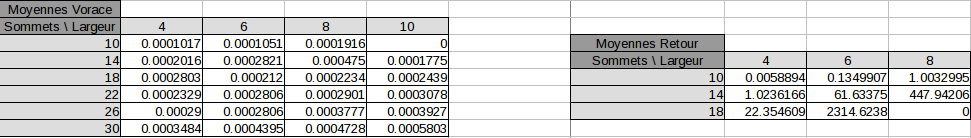
\includegraphics[width=\textwidth]{spreadsheet/temps}
	\caption{Tableau des moyennes de temps d'exécution des algorithmes vorace et retour arrière}
\end{figure} 

\begin{figure}[h!]
	\begin{subfigure}[c]{0.5\textwidth}
		\centering
		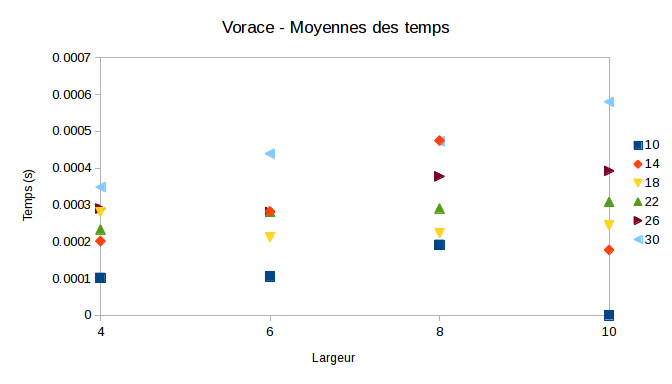
\includegraphics[width=\textwidth]{spreadsheet/graph1}
		\caption{Méthode vorace}
	\end{subfigure}
	\begin{subfigure}[c]{0.5\textwidth}
		\centering
		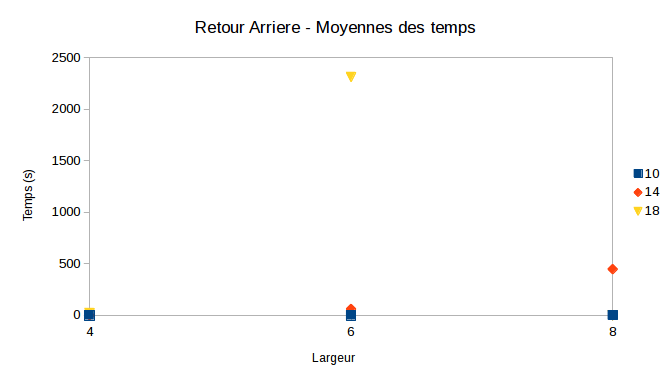
\includegraphics[width=\textwidth]{spreadsheet/graph2}
		\caption{Méthode retour arrière}
	\end{subfigure}
	\caption{Représentation graphique des moyennes de temps de calcul, selon la largeur et le nombre de sommets}
\end{figure}

Les deux graphes sont très peu similaires, même sans considérer le plus grand nombre de données du premier. L'échelle des temps d'exécution de l'algorithme retour arrière est bien plus large et croît intensément avec la largeur des exemplaires. La répartition des points sur le graphe 3.a ne permet pas de tirer de conclusion importante, si ce n'est que le temps semble croître très légèrement avec la taille de la population, et ne paraît pas être en relation avec la largeur du graphe.

Mais durant l'expérience, nous avons pu noter un très net déséquilibre des temps de calcul au sein d'une même population de résultats de l'algorithme retour arrière, ce qui ne semblait pas être le cas pour la méthode vorace. Afin d'étudier cette anomalie, nous avons calculé et reporté les écarts-type des calculs dans le tableau suivant : \\[2em]

\begin{figure}[h!]
	\centering
	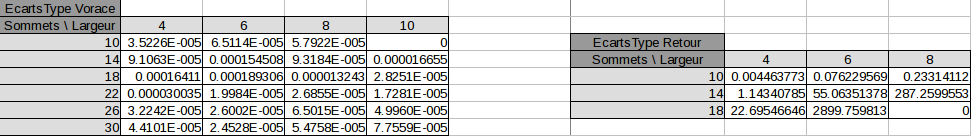
\includegraphics[width=\textwidth]{spreadsheet/ecarts}
	\caption{Tableau des écarts-type de temps d'exécution des algorithmes vorace et retour arrière}
\end{figure}

\begin{figure}[h!]
	\begin{subfigure}[c]{0.5\textwidth}
		\centering
		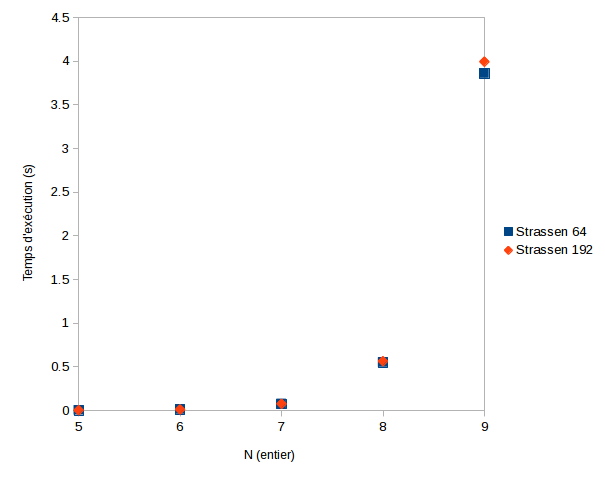
\includegraphics[width=\textwidth]{spreadsheet/graph3}
		\caption{Méthode vorace}
	\end{subfigure}
	\begin{subfigure}[c]{0.5\textwidth}
		\centering
		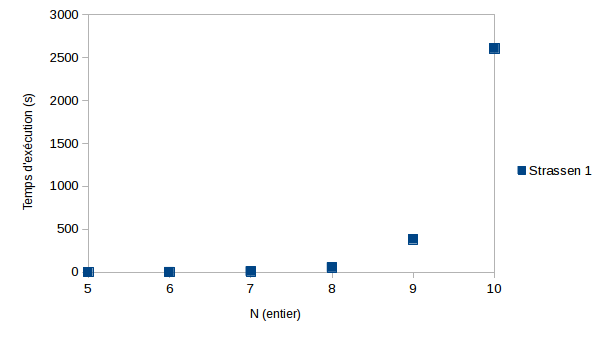
\includegraphics[width=\textwidth]{spreadsheet/graph4}
		\caption{Méthode retour arrière}
	\end{subfigure}
	\caption{Représentation graphique des écarts-type de temps de calcul, selon la largeur et le nombre de sommets}
\end{figure}

La représentation des écarts-type confirme notre impression, celui-ci semble croître exponentiellement avec la taille des exemplaires lors du calcul par \textit{backtracking}, tandis qu'il reste faible et peu significatif avec la méthode vorace.

Bien que la méthode vorace soit manifestement bien plus rapide, elle repose sur une approximation mathématique du résultat réel. Nous avons donc jugé intéressant d'étudier la marge d'erreur de cette approximation par rapport au résultat exact fourni par la méthode retour arrière. La totalité du tableau est consultable en annexe. Une partie des données est corrompue par le problème d'overflow évoqué précédemment.

Le tableau d'erreur à été calculé en confrontant nos résultats à ceux fournis sur Moodle.

\begin{figure}[h!]
	\centering
	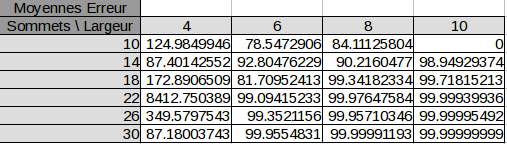
\includegraphics[width=0.7\textwidth]{spreadsheet/erreurs}
	\caption{Tableau des erreurs d'approximation des dénombrements, en \%}
\end{figure}

Dans quelques rares cas, l'approximation s'est approchée du résultat réel avec moins de 1\% d'erreur. Cependant, la tendance générale montre que les résultats approximés sont éloignés du résultat réel (ou que l'algorithme a été mal implémenté, mais ce constat est manifestement partagé par d'autres groupes d'expérience).

\section{Analyse}

\subsection{Analyse asymptotique}

\subsubsection{Algorithme vorace}

Lors de la recherche d'une chaîne la plus longue, le pire cas surviendrait si tous les sommets sauf un étaient connectés seulement à ce dernier. La file contiendrait alors $ |S| - 1 $ éléments. L'ajout / retrait dans une file est trivial et se déroule en $ O(1) $. La recherche d'élément est plus problématique, une file n'étant pas triée, et cette vitesse dépendra donc de l'implémentation. Afin de simplifier l'ajout et le retrait d'élément, et utilisation comme file (avec ajout en avant ou en fond de file) tout en gardant une structure itérable, une liste chaînée est utilisée, dans laquelle la recherche s'effectue en $ O(n) $ selon la méthode \textit{find} de la STL.

Notons que s'il n'y a aucun arc dans le graphe, nous aurons un tour de boucle de file supplémentaire, mais la recherche dans la structure n'est plus effectuée, et l'opération est plus rapide, avec un corps de boucle alors en $ O(1) $. 
Pour trouver toutes les chaînes, on répète la recherche de la chaîne la plus longue jusqu'à ce qu'il n'y ait plus de chaîne valide, soit au maximum $ |S| $ fois.
Cette méthode a donc une complexité polynomiale, en $ O(|S|^{2}) $.

\subsubsection{Algorithme retour arrière}

Cette méthode teste toutes les permutations possibles de manière exhaustive, et est donc en temps super-polynomial, appartenant à $ O (|S|!) $.

\subsubsection{Algorithme dynamique}

Rappelons le, l'algorithme dynamique consiste majoritairement à remplir un tableau n-dimensionnel de solutions de sous-problèmes et en recombiner les résultats sans effectuer de calcul redondant. Nous ne considérons pas les problématiques de complexité spatiale dans cette expérience, et laissons donc de côté les problématiques de stockage introduites par une structure de données en N dimensions.

Chaque case de cet hypercube est calculée à l'aide d'appels à la décomposition vorace d'un sous graphe. Le temps sera exponentiel.

\subsection{Analyse hybride}

Du fait des multiples variables en jeu (largeur de graphe et nombre de sommets), nous n'avons pas su comment adapter les méthodes d'analyse hybride vues précédemment. Nous avons tout de même tenté d'extraire des tendances des résultats, comme présentées sur les figures 7 et 8.

\begin{figure}[h!]
	\centering
	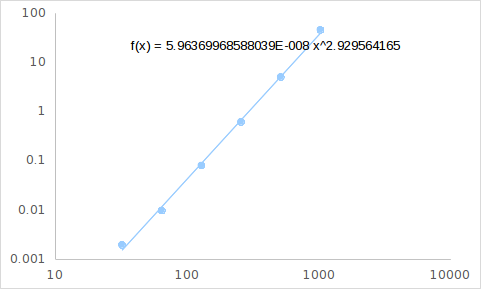
\includegraphics[width=0.7\textwidth]{spreadsheet/graph5}
	\caption{Regressions linéaires sur 3 échantillons de sommets, algorithme vorace}
\end{figure}

Les résultats de cet algorithme sont si faibles en temps d'exécution et si disparates qu'utiliser une échelle log-log est gênant pour leur visualisation.

\begin{figure}[h!]
	\centering
	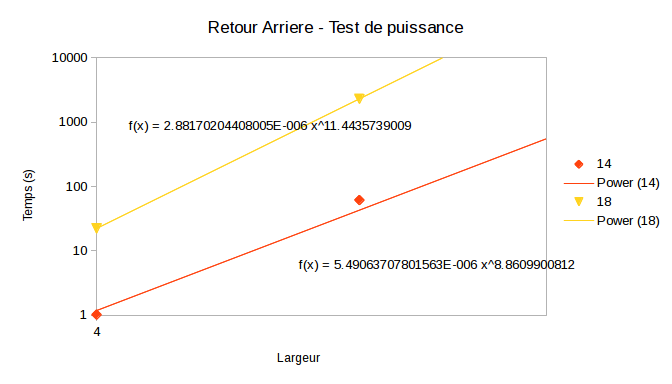
\includegraphics[width=0.7\textwidth]{spreadsheet/graph6}
	\caption{Regressions linéaires sur 2 échantillons de sommets, algorithme retour arrière}
\end{figure}

Ces graphiques semblent confirmer le comportement polynomial de la méthode vorace, avec une croissance faible, et la complexité super-polynomiale de la méthode de backtracking, avec une croissance très élevée.

\subsection{Discussion}

\subsubsection{Qualité de réponse}

Comme vu précédemment, l'approximation mathématique par l'algorithme vorace rend des solutions éloignées du résultat réel. Cette méthode peut donc seulement être utilisée afin d'avoir un ordre de grandeur rapide et efficace du résultat, sur des graphes de taille réduite, et trouve son sens par exemple dans un programme embarqué.

L'algorithme retour arrière permet d'obtenir des résultats exacts. Nous supposons aussi que la méthode dynamique fait de même, mais nous ne pouvons malheureusement pas le vérifier.

\subsubsection{Consommation de ressources}

Sans surprise, l'algorithme vorace est le plus économe en ressources. Il ne requiert qu'une map et une file, toutes deux de taille inférieure ou égale à $ |S| $.

Le \textit{backtracking} est extrêmement lourd, car il nécessite l'instanciation de deux nouveaux vecteurs de taille inférieure ou égale à $ |S| $ pour chaque embranchement, qu'il ne peut pas détruire avant d'avoir le résultat du graphe courant. Il a donc deux tableaux pour chacune des permutations possibles de sommets, soit $ 2 |S| \times |S|!$.

Quant à la méthode dynamique, elle requiert par définition l'instanciation et l'utilisation d'un tableau dont la dimension peut varier de 1 à $|S|$, et le stockage des chaînes calculées. L'initialisation du tableau est lourde et complexe, mais celui-ci peut ensuite être partagé par tous les embranchements de récursion (passage par référence). Il demande donc un espace mémoire conséquent, mais ne répète pas de nouvelles instanciations, contrairement à la méthode par retour arrière.

\subsubsection{Implémentation}

La difficulté d'implémentation des algorithmes vorace et retour arrière a été assez similaire, et moyenne. La méthode vorace requiert des choix plus réfléchis des structures de données à utiliser pour garder l'idée du pseudo-code (mécanisme de file) tout en permettant une certaine flexibilité de manipulation. La recherche d'élément, par exemple, est impossible dans une simple file. De plus, le stockage des prédecesseurs doit tenir compte du fait que le graphe peut avoir perdu de ses sommets, d'où l'intérêt d'une structure mappée.
Un autre point à souligner concernant l'implémentation de la méthode vorace est le besoin d'utiliser une formule mathématique avec des nombres extrèmement grands, de l'ordre de $10^{19}$. Cela est complètement bloquant avec la majorité des librairies standards, et demande donc la recherche et l'utilisation de librairies tierces plus adaptées.

Le retour arrière présente des problèmes plus conceptuels, sur l'utilisation de la récursion pour parcourir l'arbre de solutions, sans le avoir à le créer. Mais une fois cet écueil franchi, le reste de l'implémentation est simple.

Enfin, la méthode dynamique a posé beaucoup de problèmes sur son implémentation, uniquement à cause de l'utilisation et du parcours d'une structure de données à dimension variable. De plus, celle-ci repose sur le fait que la méthode vorace ait déjà été implémentée. C'est donc la méthode la plus complexe à concevoir et mettre en place.

\section{Conclusion}

À travers cette expérience, qui a consisté en l'étude de l’implémentation en C++ de trois méthodes de dénombrement d'extensions linéaires d'un graphe orienté acyclique, nous avons pu étudier les problématiques posées par les patrons de conception vorace, retour arrière et dynamique.

Les données recueillies après test sur jeux de données de taille variable (10 sommets, largeur 4 à 30 sommets, largeur 10) ont permis de tester les qualités de réponses des méthodes, et leur difficulté d'implémentation.

Malheureusement, cette expérience a été moins bien gérée que la précédente. Le temps demandé par l'implémentation de l'algorithme dynamique, qui ne fonctionne pas encore à ce jour, a largement retardé l'acquisition et l'analyse de résultats.

La constitution d'un nouveau binôme pour la prochaine et dernière expérience veillera à éviter cet écueil majeur.

\section{Bibliographie}

Aucune portion de code de l'implémentation ou de la représentation des résultats n'a été copié. Cependant, diverses inspirations ont permis la réalisation de cette expérience.

\begin{itemize}
	\item \href{http://msdn.microsoft.com/en-us/library/296az74e.aspx}{Microsoft Developer Network, Integer Limits}
	\item \href{http://www.cplusplus.com/reference/algorithm/find/}{C++ Reference, Find algorithm}
	\item Notes de cours "Algorithmes Voraces", Gilles Pesant
	\item Notes de cours "Algorithmes Dynamiques", Gilles Pesant
\end{itemize}

\end{document}
